\documentclass{article}

\usepackage[italian]{babel}
\usepackage[hidelinks]{hyperref}
\usepackage{graphicx}
\usepackage{listings}
\usepackage{xcolor}
\usepackage{mfirstuc}
\usepackage{calc}

\definecolor{codegreen}{rgb}{0,0.6,0}
\definecolor{codegray}{rgb}{0.5,0.5,0.5}
\definecolor{codepurple}{rgb}{0.58,0,0.82}
\definecolor{backcolour}{rgb}{0.92,0.92,0.92}

\lstdefinestyle{mystyle}{
	backgroundcolor=\color{backcolour},
	commentstyle=\color{codegreen},
	keywordstyle=\color{blue},
	numberstyle=\tiny\color{codegray},
	stringstyle=\color{codepurple},
	basicstyle=\ttfamily\footnotesize,
	breakatwhitespace=false,
	breaklines=true,
	captionpos=b,
	keepspaces=true,
	numbers=left,
	numbersep=5pt,
	showspaces=false,
	showstringspaces=false,
	showtabs=false,
	tabsize=2
}

\lstset{style=mystyle}

\graphicspath{ {./images/} }

\newcommand{\sqlinputlisting}[2]{
	\lstinputlisting[language=SQL, captionpos=t, caption={#2}]{#1}
}

% File name without extension
\newcommand{\sql}[1]{
	\sqlinputlisting{../src/#1.sql}
	{\texttt{#1.sql}}
}

\title{
	faDBula \\
	\textbf{\large
		Relazione del progetto per l'insegnamento di \break
		Basi di dati
	}
}

\author{
	Ilaria Volpe (\#766012,
	\href{mailto:ilaria.volpe2@studio.unibo.it}{ilaria.volpe2@studio.unibo.it}),
	\\
	Stefano Volpe (\#969766,
	\href{mailto:stefano.volpe2@studio.unibo.it}{stefano.volpe2@studio.unibo.it})
}

\date{
	Alma Mater Studiorum - Universit\`a di Bologna \\
	\today
}

\begin{document}

\maketitle
\thispagestyle{empty}
\pagebreak
\tableofcontents
\pagebreak
\section{Analisi dei requisiti}

\subsection{Requisiti espressi in linguaggio naturale}

Si desidera progettare una base di dati per gli appassionati di una specifica
produzione narrativa letteraria, cinematografica e/o televisiva. Lo scopo è
quello di permettere una facile analisi di trame anche complesse. Si intende
rappresentarne con codice univoco agenti, tempi, luoghi, eventi della fabula,
nonché unità narrative (anacronie e non) dell'intreccio. Sono memorizzati nome,
immagine descrittiva, sesso, momenti di nascita e di morte degli agenti. I
tempi sono rappresentati da intervalli (lineari) o da fasi (di un ciclo): dei
primi sono memorizzati l'istante di inizio e l'istante di fine mentre delle
seconde, il cui codice è progressivo, il nome. I luoghi sono caratterizzati da
nome e coordinate su una data mappa. Le mappe sono descritte da nome, immagine
ed estensione. Gli eventi sono caratterizzati da veridicità, agenti coinvolti,
luogo e intervallo. Uno o più agenti, per un dato intervallo di tempo, possono
pensare che un evento sia avvenuto. Le unità narrative sono descritte da indice,
titolo e intervallo narrato.

\subsection{Glossario dei termini}

Data la specificità del gerco in questione, non sono stati individuati sinonimi
nei requisiti espressi in linguaggio naturale.

\begin{center}\begin{tabular}{|p{0.2\textwidth-2\tabcolsep-1.2\arrayrulewidth}|p{0.55\textwidth-2\tabcolsep-1.2\arrayrulewidth}|p{0.22\textwidth-2\tabcolsep-1.2\arrayrulewidth}|}
		\hline
		\textbf{Termine} & \textbf{Descrizione}                                                                                & \textbf{Collegamenti} \\
		\hline
		Agente           & Personaggio o alias di un personaggio presente nella produzione narrativa                           & Evento                \\
		\hline
		Tempo            & Periodo temporale che occorre una o più volte nella produzione narrativa                            & Evento                \\
		\hline
		Intervallo       & Tempo di tipo lineare                                                                               & Evento                \\
		\hline
		Fase             & Tempo che ricorre una o più volte, ciclicamente                                                     & Evento                \\
		\hline
		Luogo            & Luogo presente nella produzione narrativa in cui possono avvenire eventi                            & Evento, Mappa         \\
		\hline
		Mappa            & Rappresentazione grafica in cui collocare uno o più luoghi                                          & Luogo                 \\
		\hline
		Evento           & Ciò che avviene o è pensato essere avvenuto nella produzione narrativa                              & Agente, Luogo, Tempo  \\
		\hline
		Credenza         & L'atto, da parte di uno o più agenti, di pensare che un evento sia avvenuto                         & Agente, Evento        \\
		\hline
		Unità narrativa  & Elemento della produzione narrativa che include parte, uno o più tempi                              & Tempo                 \\
		\hline
		Fabula           & Elenco degli eventi ordinati cronologicamente rispetto al momento in cui avvengono nella narrazione & Tempo, Intreccio      \\
		\hline
		Intreccio        & Elenco degli eventi ordinati cronologicamente rispetto al momento in cui sono narrati               & Tempo, Fabula         \\
		\hline
	\end{tabular}\end{center}

\subsection{Strutturazione dei requisiti}

\begin{itemize}
	\item \textbf{Frasi di carattere generale}
	      Si desidera progettare una base di dati per gli appassionati di una
	      specifica produzione narrativa letteraria, cinematografica e/o
	      televisiva. Lo scopo è quello di permettere una facile analisi di trame
	      anche complesse. Si intende rappresentarne con codice univoco agenti,
	      tempi, luoghi, eventi della fabula, nonché unità narrative (anacronie e
	      non) dell'intreccio.
	\item \textbf{Frasi relative agli agenti:}
	      Sono memorizzati nome, immagine descrittiva, sesso, momenti di nascita e
	      di morte degli agenti.
	\item \textbf{Frasi relative ai tempi:}
	      I tempi sono rappresentati da intervalli (lineari) o da fasi (di un
	      ciclo): dei primi sono memorizzati l'istante di inizio e l'istante di
	      fine mentre delle seconde, il cui codice è progressivo, il nome.
	\item \textbf{Frasi relative ai luoghi:}
	      I luoghi sono caratterizzati da nome e coordinate su una data mappa.
	\item \textbf{Frasi relative alle mappe:}
	      Le mappe sono descritte da nome, immagine ed estensione.
	\item \textbf{Frasi relative agli eventi:}
	      Gli eventi sono caratterizzati da veridicità, agenti coinvolti, luogo e
	      intervallo. Uno o più agenti, per un dato intervallo di tempo, possono
	      pensare che un evento sia avvenuto.
	\item \textbf{Frasi relative alle unità narrative:}
	      Le unità narrative sono descritte da indice, titolo e intervallo
	      narrato.
\end{itemize}

\subsection{Specifica operazioni}
Si scelgono le frequenze assumendo di tracciare una produzione narrativa
televisiva composta da 4 stagioni da 12 episodi l'una.
\begin{enumerate}
	\item Inserire un nuovo agente (in media 8 volte al mese)
	\item Inserire un nuovo intervallo (in media 80 volte al mese)
	\item Inserire una nuova fase (in media 2 volte al mese)
	\item Inserire un nuovo luogo (in media 7 volte al mese)
	\item Inserire una nuova mappa (in media 1 volta al mese)
	\item Inserire un nuovo evento (in media 160 volte al mese)
	\item Inserire una nuova unità narrativa (in media 4 volte al mese)
	\item Dato un agente, visualizzarne tutti gli alias (in media 8 volte al
	      mese)
	\item Dato un istante, visualizzare tutti gli agenti indicando se in vita o
	      meno (in media 4 volte al mese)
	\item Dato un luogo, visualizzare tutti quelli presenti nella stessa mappa (in
	      media 7 volte al mese)
	\item Dato un agente, visualizzare tutte le sue false credenze ordinate
	      cronologicamente (in media 1 volta al mese)
	\item Dato un agente e un evento, visualizzare eventuali intervalli di
	      tempo in cui il primo crede che sia avvenuto il secondo (in media 4
	      volte al mese)
	\item Visualizzare la fabula (in media 1 volta al mese)
	\item Visualizzare l'intreccio (in media 1 volta al mese)
\end{enumerate}


\section{Progettazione concettuale}

\subsection{Identificazione delle entità e relazioni (bottom-up)}
Si identificano le seguenti entità: personaggio, alias, intervallo,
fase, luogo, mappa, evento e unità narrativa.
Le prime due entità sono generalizzabili nell'entità agente.
\subsection{Un primo scheletro dello schema (top-down)}
%\begin{figure}
\includegraphics[width=\linewidth]{primo-scheletro.eps}
%\end{figure}
Un primo scheletro di schema concettuale è composto da quattro entità (agente,
intervallo, luogo, evento) e quattro relazioni. La relazione \emph{chi}
specifica quale agente partecipi all'evento, la relazione \emph{quando}
specifica a quale intervallo o fase appartenga l'evento, la relazione
\emph{dove} specifica in quale luogo avvenga l'evento e la relazione
\emph{credenza} descrive l'agente che crede all'evento per l'intervallo.
\subsection{Sviluppo delle componenti dello scheletro (inside-out)}
%\begin{figure}
\includegraphics[width=\linewidth]{agente-scheletro.eps}
%\end{figure}
%\begin{figure}
\includegraphics[width=\linewidth]{intervallo-scheletro.eps}
%\end{figure}
%\begin{figure}
\includegraphics[width=\linewidth]{luogo-scheletro.eps}
%\end{figure}
%\begin{figure}
\includegraphics[width=\linewidth]{evento-scheletro.eps}
%\end{figure}
\subsection{Unione delle componenti nello schema finale ridotto}
%\begin{figure}
\includegraphics[width=\linewidth]{schema-finale.eps}
%\end{figure}
\subsection{Dizionario dei dati}

\begin{center}\begin{tabular}{|p{0.2\textwidth-2\tabcolsep-1.2\arrayrulewidth}|p{0.4\textwidth-2\tabcolsep-1.2\arrayrulewidth}|p{0.2\textwidth-2\tabcolsep-1.2\arrayrulewidth}|p{0.2\textwidth-2\tabcolsep-1.2\arrayrulewidth}|}
		\hline
		\textbf{Nome entità} & \textbf{Descrizione}                                                               & \textbf{Attributi}                                                                                               & \textbf{Identificatore}                                     \\
		\hline
		Agente               & Personaggio o alias di un personaggio presente nella produzione narrativa          & Nome (stringa), Immagine (blob), Sesso (stringa), Istante di nascita (data e ora), Istante di morte (data e ora) & Codice (intero)                                             \\
		\hline
		Personaggio          & Personaggio presente nella produzione narrativa                                    & `` ''                                                                                                            & `` ''                                                       \\
		\hline
		Alias                & Alias di un personaggio presente nella produzione narrativa                        & `` ''                                                                                                            & `` ''                                                       \\
		\hline
		Intervallo           & Periodo temporale che occorre una volta nella produzione narrativa                 & Nome (stringa)                                                                                                   & Istante di inzio (data e ora), Istante di fine (data e ora) \\
		\hline
		Fase                 & Periodo temporale che occorre più volte ciclicamente nella produzione narrativa    & Nome (stringa)                                                                                                   & Indice (intero)                                             \\
		\hline
		Unità narrativa      & Elemento della produzione narrativa che include parte, uno o più periodi temporali & Titolo (stringa)                                                                                                 & Indice (intero)                                             \\
		\hline
		Luogo                & Luogo presente nella produzione narrativa                                          & Nome (stringa)                                                                                                   & X (reale), Y (reale), Mappa (entità in relazione)           \\
		\hline
		Mappa                & Rappresentazione grafica di uno o più luoghi presenti nella produzione narrativa   & Nome (stringa), Immagine (blob), Larghezza (reale), Altezza (reale)                                              & Codice (intero)                                             \\
		\hline
		Evento               & Ciò che avviene o è pensato essere avvenuto nella produzione narrativa             & Nome (stringa), Veridicità (booleano)                                                                            & Codice (intero)                                             \\
		\hline
	\end{tabular}\end{center}

\begin{center}\begin{tabular}{|p{0.3\textwidth-2\tabcolsep-1.2\arrayrulewidth}|p{0.2\textwidth-2\tabcolsep-1.2\arrayrulewidth}|p{0.3\textwidth-2\tabcolsep-1.2\arrayrulewidth}|p{0.2\textwidth-2\tabcolsep-1.2\arrayrulewidth}|}
		\hline
		\textbf{Nome relazione} & \textbf{Descrizione}                                                    & \textbf{Entità coinvolte}   & \textbf{Attributi}  \\
		\hline
		Mascheramento           & Associa a ogni alias uno o più personaggi                               & Personaggio, Alias          & -                   \\
		\hline
		Chi                     & Può associare eventi e agenti che vi partecipano                        & Agente, Evento              & -                   \\
		\hline
		Inclusione temporale    & Può associare fasi e intervalli che vi appartengono                     & Intervallo, Fase            & Iterazione (intero) \\
		\hline
		Narrazione              & Associa a ogni intervallo una o più unità narrative                     & Intervallo, Unità narrativa & -                   \\
		\hline
		Quando                  & Associa a ogni evento uno o più intervalli                              & Intervallo, Evento          & -                   \\
		\hline
		Collocazione            & Associa a ogni luogo una mappa                                          & Luogo, Mappa                & -                   \\
		\hline
		Dove                    & Associa a ogni evento uno o più luoghi                                  & Luogo, Evento               & -                   \\
		\hline
		Credenza                & Può associare eventi e agenti che vi credono per un intervallo di tempo & Agente, Intervallo, Evento  & -                   \\
		\hline
	\end{tabular}\end{center}


\subsection{Regole aziendali}
\begin{center}\begin{tabular}{ |l| }
		\hline
		\textbf{Regole di vincolo}                                                          \\
		\hline
		$ RV1: Agente.Sesso = M \lor Agente.Sesso = F $                                     \\
		\hline
		$RV2: Fase.Indice \geq 1 $                                                          \\
		\hline
		$RV3: InclusioneTemporale.Iterazione \geq 1 $                                       \\
		\hline
		$RV4: 0 \leq Luogo.X \leq 1 $                                                       \\
		\hline
		$RV5: 0 \leq Luogo.Y \leq 1 $                                                       \\
		\hline
		$RV6: Mappa.Larghezza > 1 $                                                         \\
		\hline
		$RV7: Mappa.Altezza > 1 $                                                           \\
		\hline
		$RV8:$ UnitàNarrativa.Indice rispetta l'espressione regolare \verb|\d+(\.\d+)*| \\
		\hline
		\textbf{Regole di derivazione}                                                      \\
		\hline
		$RD1: InVita:  = Agente.IstanteDiNascita \leq Istante \leq Agente.IstanteDiMorte$   \\
		\hline
	\end{tabular}\end{center}

\section{Progettazione logica}

\subsection{Tavole dei volumi e delle operazioni}

Si scelgono i volumi assumendo di tracciare una produzione narrativa
televisiva composta da 4 stagioni da 12 episodi l'una.

\subsubsection{Tavola dei volumi}

\begin{center}\begin{tabular}{ |c|c|c| }
		\hline
		\textbf{Concetto} & \textbf{Tipo} & \textbf{Volume} \\
		\hline
		Agente            & E             & 96              \\
		\hline
		Personaggio       & E             & 48              \\
		\hline
		Alias             & E             & 48              \\
		\hline
		Intervallo        & E             & 960             \\
		\hline
		Fase              & E             & 24              \\
		\hline
		Unità narrativa   & E             & 48              \\
		\hline
		Luogo             & E             & 84              \\
		\hline
		Mappa             & E             & 12              \\
		\hline
		Evento            & E             & 1920            \\
		\hline
	\end{tabular}\end{center}

\subsubsection{Tavola delle operazioni}

\begin{center}\begin{tabular}{ |c|c| }
		\hline
		\textbf{Operazione} & \textbf{Frequenza} \\
		\hline
		1                   & 8 volte al mese    \\
		\hline
		2                   & 80 volte al mese   \\
		\hline
		3                   & 2 volte al mese    \\
		\hline
		4                   & 7 volte al mese    \\
		\hline
		5                   & 1 volta al mese    \\
		\hline
		6                   & 160 volte al mese  \\
		\hline
		7                   & 4 volte al mese    \\
		\hline
		8                   & 8 volte al mese    \\
		\hline
		9                   & 4 volte al mese    \\
		\hline
		10                  & 7 volte al mese    \\
		\hline
		11                  & 1 volta al mese    \\
		\hline
		12                  & 4 volte al mese    \\
		\hline
		13                  & 1 volta al mese    \\
		\hline
		14                  & 1 volta al mese    \\
		\hline
	\end{tabular}\end{center}

\subsection{Ristrutturazione dello schema concettuale}

\subsubsection{Eliminazione delle ridondanze}

Il nostro modello attuale chiaramente non prevede ridondanze dovute ad attributi
derivabili: l'unica regola di derivazione che abbiamo definito computa
un'informazione non memorizzata nella base di dati, e nessun attributo memorizza
dati calcolabili dal corpo di alcuna tabella (come conteggi o risultati di altre
funzioni di aggregazione). Anche se alcune chiavi primarie contenenti
informazioni significative di fatto sono ripetute in altre tabelle come chiavi
esterne, il loro uso è comunque preferibile all'adozione di altri codici
identificativi arbitrari. Inoltre, non sono previste relazioni derivabili dalla
commposizione di altre relazioni: infatti, nessun ciclo del diagramma permette
di raggiungere un'entità a partire da un'altra tramite più percorsi distinti
senza differenze semantiche. Ne concludiamo quindi che non sono presenti
ridondanze di alcun tipo, e che non sono quindi necessarie tavole degli accessi.

Rimane da chiedersi se sia opportuno aggiungere nuove ridondanze al fine di
migliorare le operazioni di alcune operazioni tramite risultati precalcolati.
Nessuna delle operazioni specificate sopra richiede risultati (intermedi o
finali) specificabili in un unico attributo. Per esempio, per nessuna delle
operazioni è richesto il calcolo di un conteggio, o il confronto con un massimo.
Non porterebbe quindi ad alcun beneficio aggiungere singoli attributi
ridondanti. Aggiungere delle relazioni aggiuntive potrebbe invece velocizzare
le operazioni 13 e 14, che sono le uniche a richiedere una composizione di
relazioni per essere elaborate. Essendo queste operazioni non parametriche,
però, ristrutturare il modello diventa superfluo: la stragrande maggioranza dei
DBMS attuali può direttamente fare uso di viste in sola lettura.

\subsubsection{Eliminazione delle gerarchie}

L'unica gerarchia presente nel modello è la generalizzazione di ``Agente'' come
genitore di ``Personaggio'' e ``Alias''. Dal momento che nessuna delle operazioni fa
riferimento esplicito a una particolare istanziazione, a esse si fa sempre
accesso contemporaneamente, e abbiamo quindi deciso di incorporare i figli nel
genitore tramite l'aggiunta di un attributo ``Tipo'' di tipo enumerativo.

%\begin{figure}
\includegraphics[width=\linewidth]{eliminazione-gerarchie.eps}
%\end{figure}
L'unica
relazione a distinguere fra queste istanziazioni era ``Mascheramento''. Si rende
quindi necessario aggiungere due regole di vincolo che implementino un vero e
proprio ``controllo di tipo'':

\begin{math}
	RV9: Mascheramento.Personaggio.Tipo = Tipo.Personaggio
\end{math}

\begin{math}
	RV10: Mascheramento.Alias.Tipo = Tipo.Alias
\end{math}

\subsubsection{Partizionamenti e accorpamenti di entità e relazioni}

Allo stato attuale del modello, gli attributi a cui viene fatto accesso
separatamente appartengono già a entità distinte. Allo stesso modo, gli
attributi a cui viene fatto accesso contemporaneamente appartengono già alla
stessa entità. Per questi motivi, non abbiamo operato ulteriori partizionamenti
o accorpamenti.


\subsubsection{Identificazione delle chiavi primarie}

In fase di progettazione concettuale avevamo già adottato l'aggiunta di
opportuni attributi ``Codice'' qualora mancassero altri candidati a chiavi
primarie ``ragionevoli''. Questa tecnica è da considerarsi un mero ripiego di cui
non abusare.

\subsection{Normalizzazione}

\subsubsection{Entità}

Nessuna entità presenta dipendenza non banali tra i propri attributi, e quindi
tutte le entità sono necessariamente in forma normale di Boyce e Codd.

\subsubsection{Relazioni}

Oltre alle associazioni binarie, che sono necessariamente in forma normale di
Boyce e Codd, il modello include una singola relazione ternaria, che però non
presenta dipendenze non banali fra gli attributi.

\subsection{Traduzione verso il modello relazionale}

\begin{center}\begin{tabular}{|p{0.3\textwidth-2\tabcolsep-1.2\arrayrulewidth}|p{0.7\textwidth-2\tabcolsep-1.2\arrayrulewidth}|}
		\hline
		\textbf{Entità-Relazione} & \textbf{Traduzione}                                                                                  \\
		\hline
		Agente                    & Agente(\underline{Codice}, Nome, Immagine, Sesso, IstanteNascita, IstanteMorte, Tipo)                \\
		\hline
		Intervallo                & Intervallo(Nome, \underline{IstanteInizio}, \underline{IstanteFine})                                 \\
		\hline
		Fase                      & Fase(\underline{Indice}, Nome)                                                                       \\
		\hline
		Unità narrativa           & UnitàNarrativa(\underline{Indice}, Nome, \underline{IstanteInizio}, \underline{IstanteFine})         \\
		\hline
		Luogo                     & Luogo(Nome, \underline{X}, \underline{Y}, \underline{Mappa})                                         \\
		\hline
		Mappa                     & Mappa(\underline{Codice}, Nome, Immagine, Larghezza, Altezza)                                        \\
		\hline
		Evento                    & Evento(\underline{Codice}, Nome, Veridicità)                                                         \\
		\hline
		Mascheramento             & Mascheramento(\underline{Personaggio}, \underline{Alias})                                            \\
		\hline
		Chi                       & Chi(\underline{Evento}, \underline{Agente})                                                          \\
		\hline
		Quando                    & Quando(\underline{Evento}, \underline{IstanteInizio}, \underline{IstanteFine})                       \\
		\hline
		Dove                      & Dove(\underline{Evento}, \underline{X}, \underline{Y}, \underline{Mappa})                            \\
		\hline
		Credenza                  & Credenza(\underline{Evento}, \underline{Agente}, \underline{IstanteInizio}, \underline{IstanteFine}) \\
		\hline
	\end{tabular}\end{center}

\begin{center}\begin{tabular}{|p{0.6\textwidth-2\tabcolsep-1.2\arrayrulewidth}|p{0.4\textwidth-2\tabcolsep-1.2\arrayrulewidth}|}
		\hline
		\textbf{Traduzione}                                                                                  & \textbf{Vincoli di riferimento}                                                                                                                                                \\
		\hline
		Agente(\underline{Codice}, Nome, Immagine, Sesso, IstanteNascita, IstanteMorte, Tipo)                & -                                                                                                                                                                              \\
		\hline
		Intervallo(Nome, \underline{IstanteInizio}, \underline{IstanteFine})                                 & -                                                                                                                                                                              \\
		\hline
		Fase(\underline{Indice}, Nome)                                                                       & -                                                                                                                                                                              \\
		\hline
		UnitàNarrativa(\underline{Indice}, Nome, \underline{IstanteInizio}, \underline{IstanteFine})         & IstanteInizio $\rightarrow$ Intervallo.IstanteInizio, IstanteFine $\rightarrow$ Intervallo.IstanteFine                                                                         \\
		\hline
		Luogo(Nome, \underline{X}, \underline{Y}, \underline{Mappa})                                         & Mappa $\rightarrow$ Mappa.Codice                                                                                                                                               \\
		\hline
		Mappa(\underline{Codice}, Nome, Immagine, Larghezza, Altezza)                                        & -                                                                                                                                                                              \\
		\hline
		Evento(\underline{Codice}, Nome, Veridicità)                                                         & -                                                                                                                                                                              \\
		\hline
		Mascheramento(\underline{Personaggio}, \underline{Alias})                                            & Personaggio $\rightarrow$ Agente.Codice, Alias $\rightarrow$ Agente.Codice                                                                                                     \\
		\hline
		Chi(\underline{Evento}, \underline{Agente})                                                          & Evento $\rightarrow$ Evento.Codice, Agente $\rightarrow$ Agente.Codice                                                                                                         \\
		\hline
		Quando(\underline{Evento}, \underline{IstanteInizio}, \underline{IstanteFine})                       & Evento $\rightarrow$ Evento.Codice, IstanteInizio $\rightarrow$ Intervallo.IstanteInizio, IstanteFine $\rightarrow$ Intervallo.IstanteFine                                     \\
		\hline
		Dove(\underline{Evento}, \underline{X}, \underline{Y}, \underline{Mappa})                            & Evento $\rightarrow$ Evento.Codice, X $\rightarrow$ Luogo.X, Y $\rightarrow$ Luogo.Y, Mappa $\rightarrow$ Luogo.Mappa                                                          \\
		\hline
		Credenza(\underline{Evento}, \underline{Agente}, \underline{IstanteInizio}, \underline{IstanteFine}) & Evento $\rightarrow$ Evento.Codice, Agente $\rightarrow$ Agente.Codice, IstanteInizio $\rightarrow$ Intervallo.IstanteInizio, IstanteFine $\rightarrow$ Intervallo.IstanteFine \\
		\hline
	\end{tabular}\end{center}

\section{Codifica SQL}

\subsection{Definizione dello schema}

\sql{schema}

\subsection{Codifica delle operazioni}

\sql{operation-01}

\end{document}
